\parindent 0in
\parskip 0.1in

\begin{center}
{\bf Reduced Order Modeling of Heat and Fluid Flow: \\ 
Multi-Scale Modeling of Advanced Reactors to Enable Faster Deployment}
\end{center}

{\bf Technical work scope identification: M\&S 1 }

{\bf PI: }\begin{minipage}[t]{5in}
Paul Fischer \\
Department of Computer Science \\
Department of Mechanical Science \& Engineering \\
University of Illinois, Urbana-Champaign \\
\end{minipage}

{\bf co-PIs: } \begin{minipage}[t]{5in}
Elia Merzari, Pennsylvania State University \\
Dillon Shaver, Argonne National Laboratory \\[-3ex]
\end{minipage}

\section{Project Summary}

% \begin{itemize}
% \item
% A summary of the proposed project, including a description of the project and a
% {\em clear explanation of its importance and relevance to the objectives in Part I
% Section A.}
% \item
% Major deliverables and outcomes the R\&D will produce.
% \item
% Timeframe of execution: October 1, 2023--September 30, 2026
% \end{itemize}

We seek \textbf{to develop novel multi-scale algorithmic approaches for the
simulation of heat and fluid flow in advanced reactors}. The methods, which
leverage recent advances in hardware and reduced order modeling approaches,
will enable fast-running simulations of vastly accelerated speed, while
maintaining accuracy comparable to high-fidelity methods such Large Eddy
Simulation (LES) and Direct Numerical Simulation (DNS). These methods will
allow to perform
parameter sweeps to assess uncertainty and develop closures. They will also
enable, for the first time, to perform high fidelity simulation of transients.

Several  advanced reactor concepts are currently being pursued in the United
States, with dozens of companies proposing unique designs. Crucial for their
deployment is the analysis of  reactor transients (e.g., a protected loss of
flow): an essential part of the evaluation of thermal margins and the overall
safety case.  In most cases, licensing will be pursued with established
methods, based on lumped parameter system codes (e.g., SAM \cite{hu2021}).
However, these codes require adequate closures that are typically obtained
empirically and require extensive validation. Furthermore, these methods are
characterized by high level of uncertainty when dealing with complex
three-dimensional turbulent flow, especially in the presence of large
enclosures, mixed convection, and thermal stratification. High-fidelity
simulation on the other hand remains prohibitively expensive, especially for
large parameter sweeps or for the simulation of nuclear transients, and data
remains sparse.

Moreover, as the advanced reactor industry matures and moves past demonstration
projects, economics will become a larger driver. This pressure will likely push
vendors to seek to maximize the economic potential (e.g., higher power output,
higher temperature for process heat, reduced capital cost), especially as new
materials and fuels are introduced. These goals will benefit from radically
improved methods to assess thermal margins that push toward high fidelity.
\textbf{This proposal seeks to develop radically novel algorithmic approaches
to the simulation of advanced reactors, with an unprecedented level of
fidelity, enabling transformative design approaches and improved economics.} 
In particular we aim to: 
\begin{enumerate}
%
   \item \textit{Enable the simulation of large parameter sweeps using reduced
   order models developed over a subset of the parameter space.} This approach
   will allow to assess uncertainty of system-level approaches and to develop
   closures.
%
   \item \textit{Enable the accelerated simulation of transients.}
   This approach will allow to assess lower resolution approaches in conjunction
   with experimental data for the simulation of transient.  
\end{enumerate}
As a demonstration application we choose the simulation of Sodium Fast Reactor
(SFR) fuel assemblies under steady-state and transient conditions. \textit{We
emphasize that the methods developed will apply to a broad range of advanced
reactor applications.}

\begin{figure}[t!] \centering
    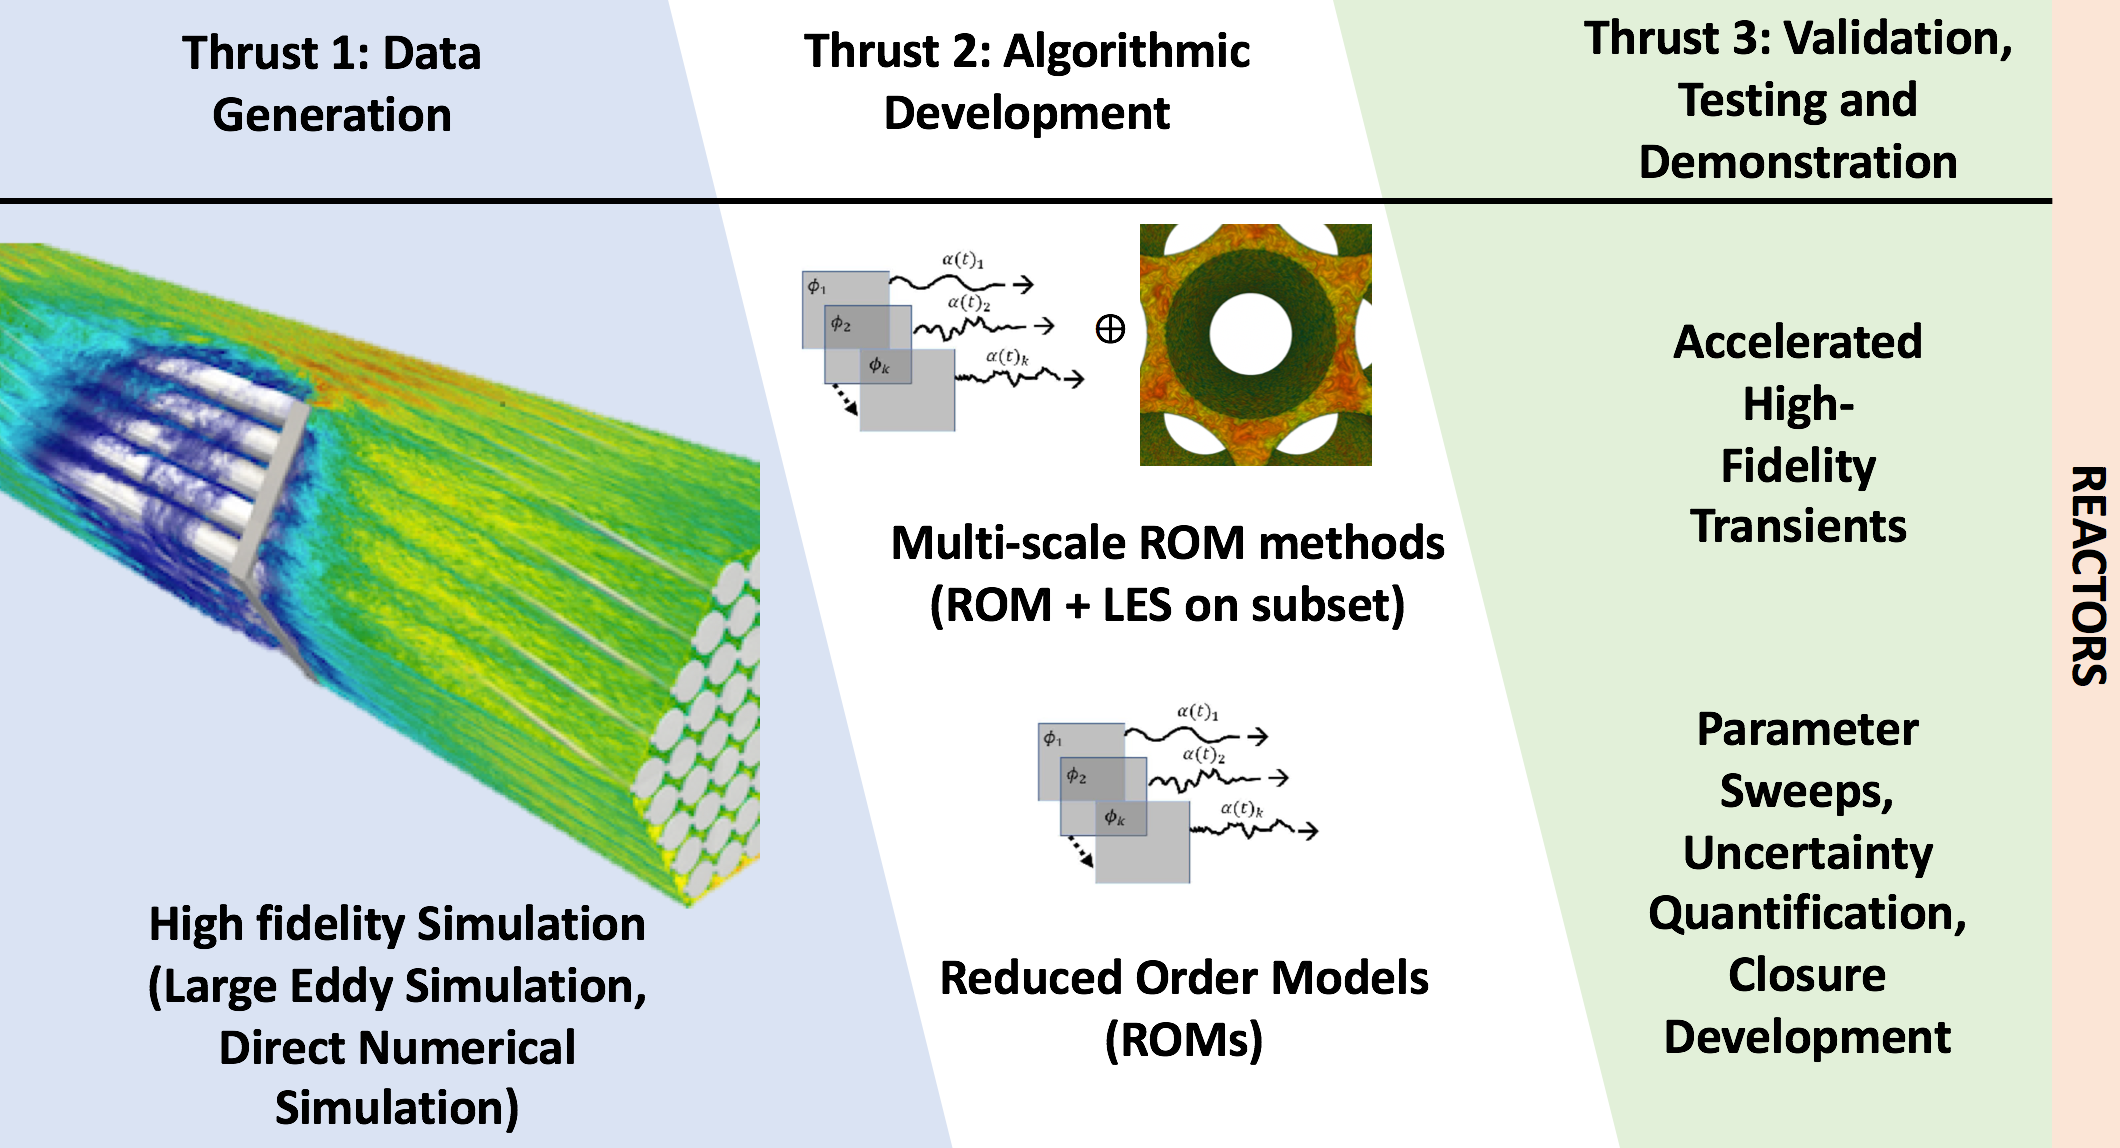
\includegraphics[width = 0.80\textwidth]{figs/overview.png}
    \caption{Overview of Project with three thrusts: Data generation,
             algorithmic development and validation/demonstration.  \label{fig:sum}}
\end{figure}


\section{Project Motivation and Technical Objectives}

We propose to leverage ongoing hardware, software, and algorithmic developments
to dramatically enhance thermal-hydraulic analysis capabilities.  The work will
entail combining advanced simulations on DOE's exascale computing platforms
with modern data analysis methods that effectively compress these
first-principle data to efficient exploratory tools based on reduced-order
models (ROMs).
We illustrate the project overview in Fig. \ref{fig:sum}.

\noindent
{\bf High-Fidelity Simulations on DOE Leadership Computers.}
The DOE is bringing several accelerator-based exascale platforms online,
including Frontier at ORNL and Aurora at ANL.  As illustrated in Fig.
\ref{fig:pbr}, we have demonstrated that it is possible to simulate a single
flow through time for the thermal-hydraulics of a full pebble-bed reactor core
(352,000 pebbles) in just six hours of wall-clock time on ORNL's {\em
pre}-exascale machine, Summit.   This is an significant acheivement as it
involves updating a quarter-trillion degrees-of-freedom at $\approx$ 0.3
seconds per step.  The software that enables this achievement is {\em NekRS},
which is the GPU-oriented version of the highly-scalable thermal-fluids code,
Nek5000.  NekRS is being developed under DOE's Center for Efficient Exascale
Discretizations (CEED) and sustains $\approx$ 0.5--1.0 TFLOPS ($10^{12}$
floating point operations per second) per MPI rank on current pre-exascale
platforms (e.g., Summit and Crusher at ORNL and Polaris at ANL).  It is a
highly efficient code that realizes 2--4 TFLOPS-FP64/rank on key kernels and
80\% parallel efficiency with about 2M grid points per rank.  Consequently, a
50B grid-point problem such as the full pebble-bed reactor core of Fig.
\ref{fig:pbr} can effectively use $P$=25,000 GPUs (or GCDs in the case of
Frontier or tiles in the case of Aurora).  While such a calculation essentially
fills all of Summit, it would use only a fraction of Frontier or Aurora.  On
these platforms, we can anticipate running larger problems or running at
multiple points in the reactor design space, where execution times can be
anticipated to remain at $\approx$ 0.1--0.3 seconds per step even with larger
problems running on the full systems.

Like Nek5000, NekRS is based on high-order body-fitted spectral element
discretizations that has minimal numerical dispersion and dissipation, which
are essential features for efficient simulation of turbulence.  Time-stepping
uses either a $k$th-order semi-implicit method ($k$=2 or 3) or a $k$th-order
characteristics scheme that allows Courant numbers significantly larger than
unity.  NekRS has an extensive suite of preconditioners for the
pressure-Poisson problem that are tailored to accelerator-based HPC platforms.
Fast Poisson solvers are critical to rapid simulation of incompressible and
weakly compressible flows.   As part of the Nek5000 source, NekRS supports all
of the features of Nek5000, which include a large variety of boundary conditions
and an extensive tool set for data analysis of turbulent heat transfer.



\begin{figure}[t!] \centering
    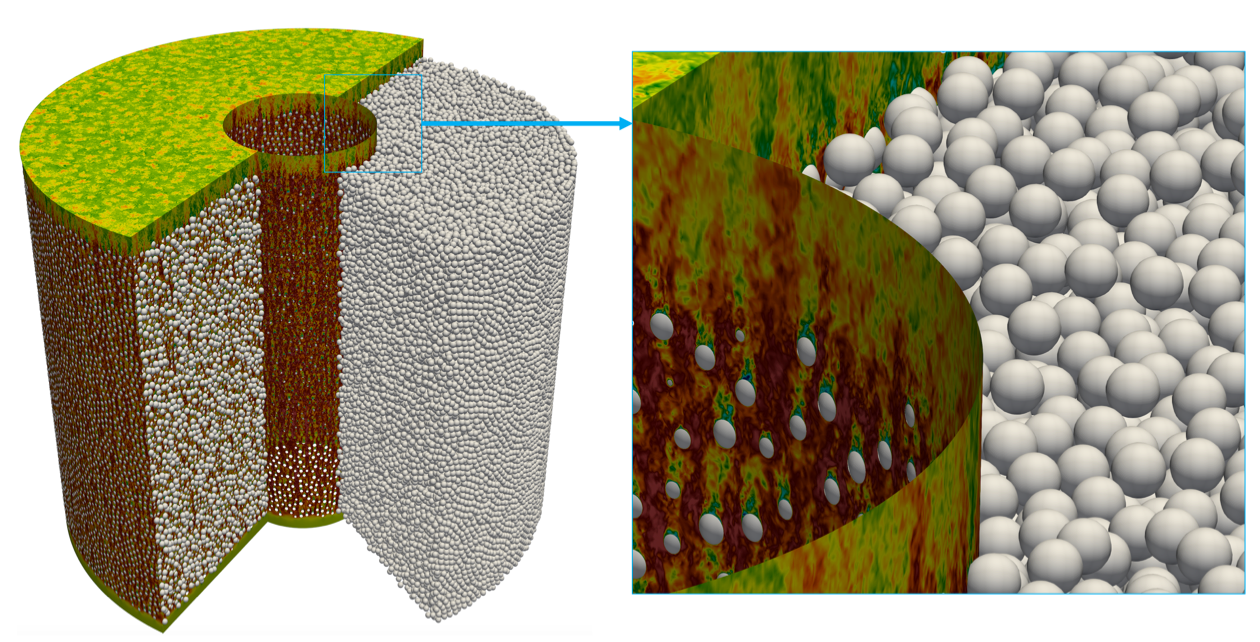
\includegraphics[width = 0.60\textwidth]{figs/pbr_pair.png}
    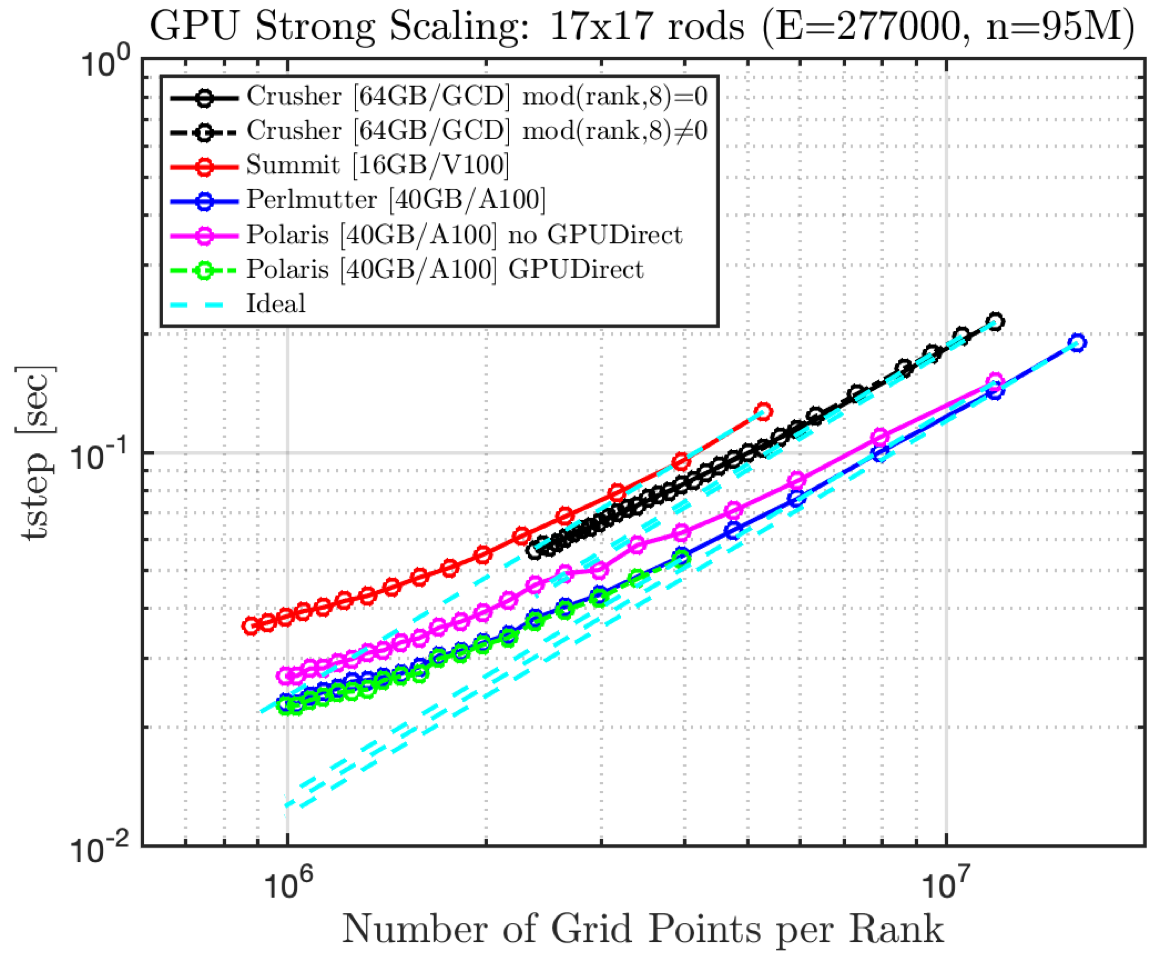
\includegraphics[width = 0.35\textwidth]{figs/nekrs_17x17_crusher_strong.png}
    \caption{(left) NekRS turbulent flow simulation results for a full reactor
core with 352625 pebbles.  The simulation comprised 51 billion gridpoints
($E$=99M spectral elements of order $p$=8).  On all of Summit (27648 NVIDIA
V100 GPUs), this simulation requires 0.36 seconds per step and would complete a
single flow-through time in just six hours \cite{sc22}. (Computation by
Yu-Hsiang Lan, ANL/UIUC.)
(right) NekRS strong-scaling on current-generation accelerator-based platforms:
AMD-MI250X-based Crusher (OLCF),
NVIDIA-V100-based Summit (OLCF),
NVIDIA-A100-based Perlmutter (NERSC),
NVIDIA-A100-based Polaris (ALCF).
The test problem is a 17$\times$17 rod-bundle with 95 million grid points.
(Simulations by Misun Min, ANL, and Yu-Hsiang Lan, ANL/UIUC.)
\label{fig:pbr}}
\end{figure}


%% (WHY ROM)
\noindent
{\bf Data-Driven Reduced-Order Models.}
While it is clear that NekRS will be capable of delivering fast turn-around
for reactor-scale simulations on DOE's exascale platforms, the use of 
such simulations for one-off determination of system behavior at a single
parameter point does not fully leverage the data generated by such a large
calculation.
From a design perspective, it is far more efficient if one can reliably
explore parametric input/output relationships (e.g., Nusselt/Rayleigh-number
relationships under low-flow conditions) in the neighborhood of the parameter
space for which the high-fidelity DNS or LES is performed.   Such a capability
is precisely the goal of parametric model-order reduction (pMOR), which is
typically based on reduced-order models (ROMs) of the high-fidelity DNS/LES
(often referred to as full-order models, or FOMs).   

Under NEUP Award 18-15520, we have developed have developed NekROM to provide a
pMOR/ROM capability within the Nek5000 framework that allows users to build
ROMs and perform parameter variation with these models.  The development of
ROMs for unsteady (e.g., turbulent or transient) flows is still an open
research topic.  In broad terms, the process consists of two problems: {\em (i)
the solution reproduction problem}, and {\em (ii) the parametric problem}.  To
these, we add a third category of relevance to the current project: {\em (iii)
evolution of long transients}.

We begin with the reproduction problem. The standard approach is to use
$K$$\approx$1000 high-fidelity solution snapshots (i.e., full velocity/temperature
fields) to form $N$$\approx$20--200 basis functions through 
proper-orthogonal decomposition (POD) or some other low-rank approximation
approach.  These bases can be used to approximate solutions to the governing
Navier-Stokes and energy-transport equations, from which one can extract a 
low-dimensional dynamical system governing the unknown basis coefficients.  
These systems, which are of size $N$, run extremely fast---in just a few
minutes on a laptop it is possible to evolve tens-of-thousands of convective
time units, much longer than feasible with a FOM, even on an exascale platform,
which is one of the reasons that ROMs are interesting for long-time transients.
Moreover, it is relatively easy to adjust equation parameters to have a nominal
pMOR tool.  (Adjusting geometry is more challenging and one of the topics to be
explored in the context of this project).

There are several challenges to bringing the preceding scenario to fruition.
The first is to ensure that the ROM can effectively track the quantities
of interest (QOIs) produced by the FOM, even at the same parameter point.
This tracking is by no means assured, particularly for turbulent flows
where energy is dissipated by small-scale structures that are generally absent
from POD bases.  Several stabilization strategies are possible, such as Leray
regularization \cite{wang2012proper} or constrained coefficient evolution
\cite{fick}.  Alternative approaches include modification of the approximation
space.  For example \cite{akkari19} uses a decomposition of modes that minimize
into distinct sets minimizing the $L^2$ error (for accuracy) and the $\cH^1$
error (for stability).  In \cite{khodkar2019} a basis is derived from Green's
functions approximations.
   Under prior NEUP support, Kaneko \cite{kaneko22a,kaneko22} developed an
augmented-basis method (ABM) wherein a set of standard POD basis functions,
$\{\bz_i(\bx) \}$,  is augmented with a subset of their nonlinear interaction
terms, $\{\bz_i \cdot \nabla \bz_j\}$.   

The success of the ABM approach is illustrated in the turbulent pipe flow
examples of Fig. \ref{fig:abm}, which shows that standard POD Galerkin
and Leray regularization can converge at lower Reynolds numbers $Re$
with a sufficient number of basis functions, $N$, but that the required
number of basis functions rapidly increases with $Re$.  Given the $O(N^3)$
costs for the ROM, these methods appear to be limited to relatively low
$Re$.  The ABM and the constrained approaches, however, perform much better
because of their stability.

\begin{figure}[t!] \centering
    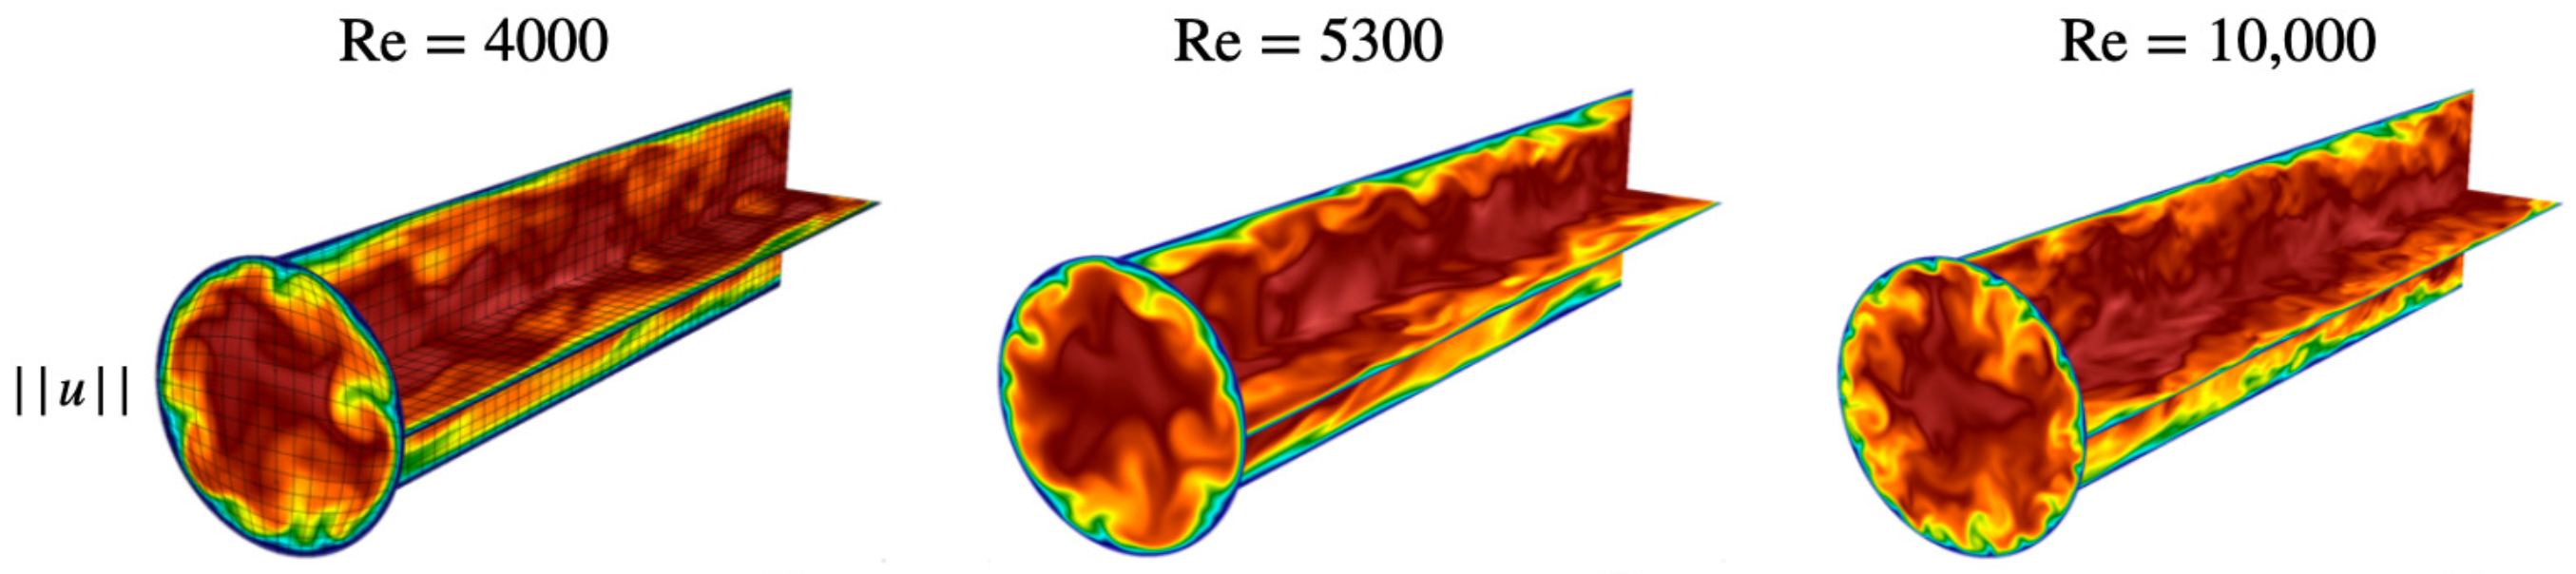
\includegraphics[width = 0.70\textwidth]{figs/kaneko_diss_pipe_pics.png}
    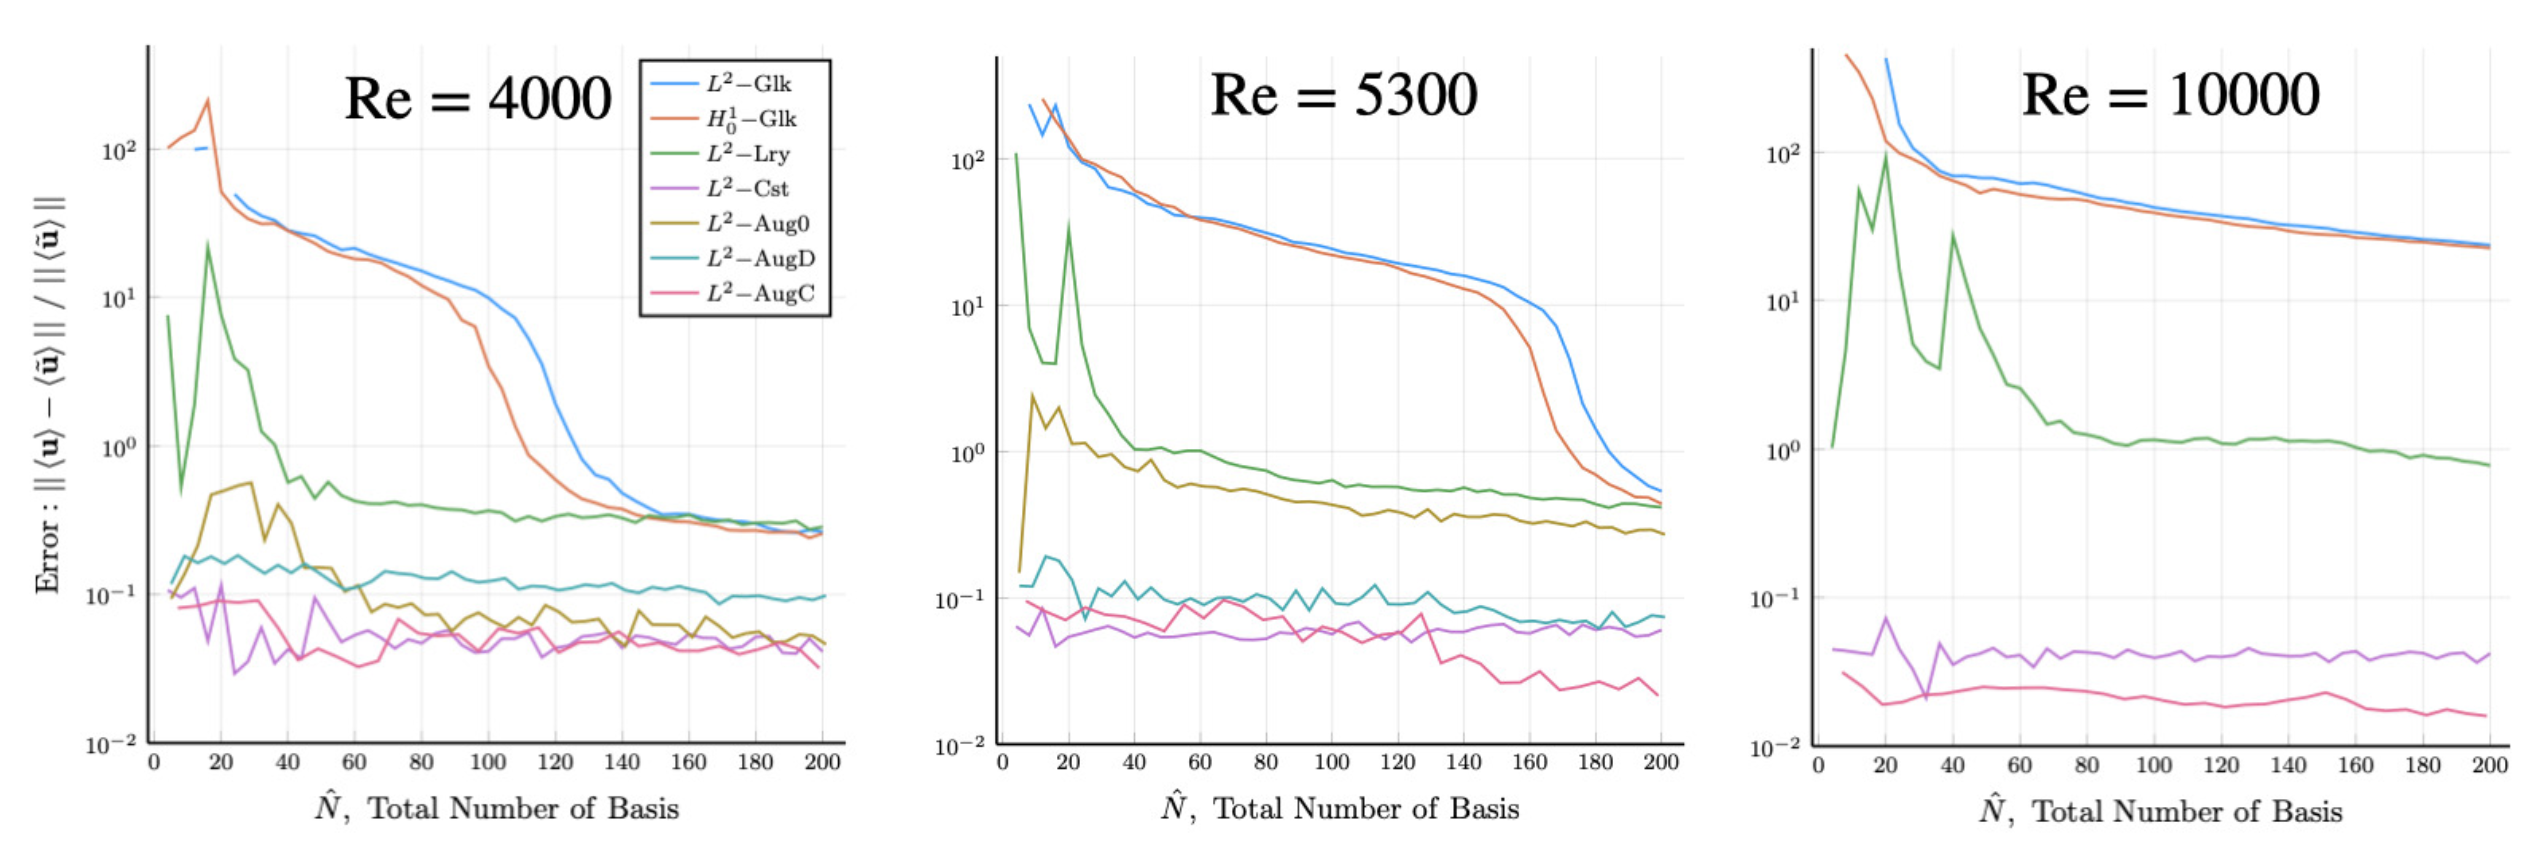
\includegraphics[width = 0.70\textwidth]{figs/kaneko_diss_pipe_ubar.png}
\caption{
(top) Nek5000 DNS of turbulent pipe flow at $Re_D$=4000--10,000;
(bottom) Mean velocity error in NekROM reproduction results for standard
Galerkin POD ($L^2$-Glk, $H^1$-Glk), 
Leray- and constrainted-based regularization
($L^2$-Lry, $H^1$-Cst), and 
ABM with three different subsets of the nonlinear terms
(L^2$-Aug0 = $ \bz_0 \cdot \nabla \bz_j+ \bz_j \cdot \nabla \bz_0$,
$L^2$-AugD = $ \bz_j \cdot \nabla \bz_j$,
$L^2$-Aug0 $\bigcup$ $L^2$-AugD) \cite{kaneko22a,kaneko22}.
\label{fig:abm}}
\end{figure}




